\documentclass[border=3pt,tikz]{standalone}
\usepackage{amsmath}
\usetikzlibrary{calc}
\usetikzlibrary{arrows.meta} % for arrow size
\begin{document}
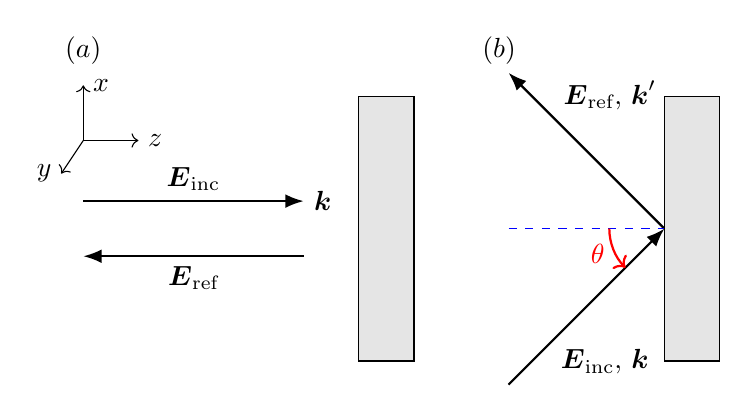
\begin{tikzpicture}[scale=1.4, rotate=0]
\begin{scope}
    \draw[->] (0, 0.8) -- (0.5, 0.8) node [right]{$z$};
    \draw[->] (0, 0.8) -- (0, 1.3) node [right]{$x$};
    \draw[->] (0, 0.8) -- (-0.2, 0.5) node [left]{$y$};

    \draw[thick, -Latex](0,0.25) -- node[above]{$\boldsymbol{E}_{\text{inc}}$}(2,0.25) node[right]{$\boldsymbol{k}$};
    \draw[thick, Latex-](0,-0.25) -- node[below]{$\boldsymbol{E}_{\text{ref}}$}(2,-0.25) ;
    \filldraw [fill=gray!20, draw=black] (2.5, 1.2) rectangle (3.0,-1.2);
    \node[above] at (0.0, 1.4) {$(a)$} ;
\end{scope}

\begin{scope}[xshift=150]
    \draw[thick, Latex-]({-sqrt(2)},{sqrt(2)}) -- node[right, yshift=2em, xshift = -1.2em]{$\boldsymbol{E}_{\text{ref}},\,\boldsymbol{k}'$}(0,0);
    \draw[thick, -Latex]({-sqrt(2)},-{sqrt(2)}) -- node[right, yshift=-2em, xshift=-1.3em]{$\boldsymbol{E}_{\text{inc}},\,\boldsymbol{k}$}(0,0) ;
    \draw[dashed, blue] ({-sqrt(2)}, 0) -- (0,0);
    \filldraw [fill=gray!20, draw=black] (0, 1.2) rectangle (0.5,-1.2);
    \node[above] at (-1.50, 1.4) {$(b)$} ;
    \draw[thick, red, ->] (-0.5,0) arc (180:225:0.5) node[yshift = 0.5em, xshift = -1em] {$\theta$};
\end{scope}
\end{tikzpicture}
\end{document}